
\documentclass[a4paper,12pt]{book}
\usepackage[font=scriptsize]{caption}
\usepackage[T1]{fontenc}
\usepackage[italian,english]{babel}
\usepackage[utf8]{inputenc}
\usepackage{graphicx}
\usepackage{grffile}
\usepackage{color}
\usepackage{float}
\usepackage{cite}
\usepackage{amsmath}
\usepackage{amssymb}
\usepackage{amsthm}
\usepackage{wasysym}
\usepackage{setspace}
\usepackage{algorithm}
\usepackage{algorithmic}
\usepackage{multirow}
\usepackage{listings}
\usepackage{url}
\usepackage[height=21.6cm,width=15cm,centering]{geometry}
\usepackage{tabularx}
\usepackage[super]{nth}

\usepackage[bookmarks=true,hyperindex,colorlinks=false,
            pdfborder={0 0 0},pdfstartview=FitH,pdfpagelayout=SinglePage,
            pdfauthor={Marco Edemanti},
            pdftitle={RASD WeatherCal},
            pdfsubject={}]{hyperref}
\makeatletter
\newcommand*{\textlabel}[2]{%
  \edef\@currentlabel{#1}% Set target label
  \phantomsection% Correct hyper reference link
  #1\label{#2}% Print and store label
}
\newcommand{\myparagraph}[1]{\paragraph{#1}\mbox{}\\}
\renewenvironment{thebibliography}[1]
     {\section{References}% <-- this line was changed from \chapter* to \section*
      \@mkboth{\MakeUppercase\bibname}{\MakeUppercase\bibname}%
      \list{\@biblabel{\@arabic\c@enumiv}}%
           {\settowidth\labelwidth{\@biblabel{#1}}%
            \leftmargin\labelwidth
            \advance\leftmargin\labelsep
            \@openbib@code
            \usecounter{enumiv}%
            \let\p@enumiv\@empty
            \renewcommand\theenumiv{\@arabic\c@enumiv}}%
      \sloppy
      \clubpenalty4000
      \@clubpenalty \clubpenalty
      \widowpenalty4000%
      \sfcode`\.\@m}
     {\def\@noitemerr
       {\@latex@warning{Empty `thebibliography' environment}}%
      \endlist}
\makeatother

\title{Testing Document WeatherCal}
\author{Edemanti Marco}
\author{Polidori Paolo}

\begin{document}
\selectlanguage{english}
\definecolor{lightgray}{rgb}{.9,.9,.9}
\definecolor{darkgray}{rgb}{.4,.4,.4}
\definecolor{purple}{rgb}{0.65, 0.12, 0.82}
\definecolor{lightgreen}{rgb}{0.06,0.60,0.34}
\lstdefinelanguage{alloy}{
  keywords={t assert, pred, all, no, lone, one, some, check, run,
      but, let, implies, not, iff, in, and, or, set, sig, Int, int,
      if, then, else, exactly, disj, fact, fun, module, abstract,
      extends, open, none, univ, iden, seq,},
  keywordstyle=\color{blue}\bfseries,
  ndkeywords={class, export, boolean, throw, implements, import, this},
  ndkeywordstyle=\color{darkgray}\bfseries,
  identifierstyle=\color{black},
  sensitive=false,
  comment=[l]{//},
  morecomment=[s]{/*}{*/},
  commentstyle=\color{lightgreen}\bfseries,
  stringstyle=\color{red}\ttfamily,
  morestring=[b]',
  morestring=[b]"
}
\setcounter{secnumdepth}{5}
\lstset{ %
  backgroundcolor=\color{white},   % choose the background color; you must add \usepackage{color} or \usepackage{xcolor}
  basicstyle=\footnotesize,        % the size of the fonts that are used for the code
  breakatwhitespace=false,         % sets if automatic breaks should only happen at whitespace
  breaklines=true,                 % sets automatic line breaking
  captionpos=b,                    % sets the caption-position to bottom
  commentstyle=\color{green},    % comment style
  deletekeywords={...},            % if you want to delete keywords from the given language
  escapeinside={\%*}{*)},          % if you want to add LaTeX within your code
  extendedchars=true,              % lets you use non-ASCII characters; for 8-bits encodings only, does not work with UTF-8
  frame=single,                    % adds a frame around the code
  keepspaces=true,                 % keeps spaces in text, useful for keeping indentation of code (possibly needs columns=flexible)
  keywordstyle=\color{blue},       % keyword style
  language=alloy,                 % the language of the code
  morekeywords={*,...},            % if you want to add more keywords to the set
  numbers=left,                    % where to put the line-numbers; possible values are (none, left, right)
  numbersep=5pt,                   % how far the line-numbers are from the code
  showspaces=false,                % show spaces everywhere adding particular underscores; it overrides 'showstringspaces'
  showstringspaces=false,          % underline spaces within strings only
  showtabs=false,                  % show tabs within strings adding particular underscores
  stepnumber=2,                    % the step between two line-numbers. If it's 1, each line will be numbered
  tabsize=2,                       % sets default tabsize to 2 spaces
}
 \begin{center}
    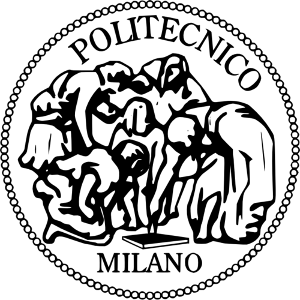
\includegraphics[width=4cm]{../RASD/immagini/polilogo.png}
    \end{center}
\begin{center}

{\huge{\bf\uppercase {Testing Document}}}


\end{center}
\vspace*{0.5cm}
\begin{center}
{\large Project of Software Engineering 2\\ \vspace*{0.5cm} \huge WEATHER-CAL}
\end{center}
\begin{flushright}
 \vspace*{9cm}

        {\bf Authors: }\\
        \vspace*{0.2cm}
            {\bf   {PAOLO POLIDORI} }\\
             \vspace*{0.3cm}
            {\bf   {MARCO EDEMANTI} }
    \end{flushright}

\doublespacing    
\tableofcontents

\chapter{Introduction} \label{cap:cap1}

\section{Purpose}
The purpose of this document is to present a description of WheaterCal system. It will explain the features of the system, the interfaces of the system, what the system will do and the constraints under which it must operate.
This document is intended for both the stakeholders and the developers of the system.
Stakeholders of the system are the client, which is our teacher and their assistants, composing the group that will evaluate our project, the testers, which are a team with our same project and our same tasks and the developers, which are the authors of this document.

\section{Scope}
We want to project and implement WheaterCal. The aim of this project is to develop a system that offers an online calendar in which user can schedule their events according to the weather conditions.\\ A registered user can create, delete and update an event and moreover he should provide information about where and when this event will take place and information about the invited user.
Once the event is created the system should provide to its creator the weather forecast information regarding the scheduled day, and most of all it should notify a bad weather condition one day in advance to all the participants.\\
Also a user is able to make his/her calendar visible to all other registered user showing them only the time slots in which they are busy without letting know the event information unless either the event is public.
In addition in case of bad weather, three day before the scheduled data of an event, the system will inform the event's owner and propose to him the closest sunny day.

\section{Glossary}
\begin{tabularx}{\linewidth}{|r|X|}
  \hline  {\bf Anonymous User} & People who access the system but didn't authenticate\\ 
  \hline  {\bf Registered User} & People who both registered to the platform and logged in. Sometimes referred to as "User"\\ 
  \hline  {\bf Platform, System} & The WeatherCal application\\
  \hline  {\bf Bad Weather}&  Undesired conditions for an event to take place basing on the event owner's choices\\
  \hline  {\bf Notification} & A message that arrives to the user in dedicated area, which can be easily identified by the user at first sight\\
  \hline  {\bf Event owner} & The user who created the event and for which is responsibile of the organization\\
  \hline  {\bf Event invited} & A user invited to an event for which can decide if he wants to be a participant or not\\
  \hline  {\bf Event participant} & A user invited to an event for which decided to participate\\
  \hline  {\bf Event} & An occurrence, which was inserted in the system which should happen in a certain date and a certain time\\
  \hline  {\bf Calendar} & The set of all the events for a user, shown in a per-month view\\
  \hline
\end{tabularx}\\
\section{References}
IEEE,{\it IEEE Std 830-1998,IEEE Recommended Practice for Software Requirements Specifications},  IEEE Computer Society 1998

 
\chapter{Testing} \label{cap:cap2}
In this section we report all the test case result according to the functional requirements specified in RASD document.

 \section{Features to be tested}
 \begin{tabularx}{\linewidth}{|r|X|X|}
  \hline  {\bf Test Case Id} &{\bf Description}\\
  \hline TC1 & Log In/Out \\
  \hline TC2 & User Registration \\
  \hline TC3 & Event Creation \\
  \hline TC4 & Event Deletion \\
  \hline TC5 & Notify Event Deletion \\
  \hline TC6 & Event Management \\
  \hline TC7 & Event Loading\\
  \hline TC8 & User Invitation \\
  \hline TC9 & Check Notifications \\
  \hline TC10 & Manage Event Visibility \\
  \hline TC11 & Manage Calendar Visibility \\
  \hline TC12 & Search an user \\
  \hline TC13 & Notify bad weather condition \\ 
  \hline TC14 & Suggest the closest day with the desired weather constraint \\
  \hline
\end{tabularx}
 
\section{Test Report and Specification}
Test cases and their results are going to be documented as follows\\
\begin{tabularx}{\linewidth}{|r|X|X|}
  \hline   {\bf Test Case Id} &  The ID or the number of the test case\\
  \hline  {\bf Goal} & Description of the test case\\
  \hline  {\bf Expected Result} & The result that should be observed from a succesfull test\\
  \hline  {\bf Actual Result} & The result which is observed after applying the test steps\\
  \hline  {\bf Conclusion} & F: Failed, N: Not tested, S: Succesful, M: manually tested\\
  \hline
\end{tabularx}

\chapter{Test Case} \label{cap:cap3}
\section{Log In/Out}
\begin{tabularx}{\linewidth}{|r|X|X|}

  \hline   {\bf Test Case Id} &  TC1\\
  \hline  {\bf Goal} & Log in to or out from the system\\
  
  \hline  {\bf Expected Result} & The system redirects the user to its home page\\
  \hline  {\bf Actual Result} & The system redirects the user to its home page\\
  \hline  {\bf Conclusion} & M\\
  \hline
  
\end{tabularx}

\section{Sign In}
\begin{tabularx}{\linewidth}{|r|X|X|}

  \hline   {\bf Test Case Id} &  TC2\\
  \hline  {\bf Goal} & Sign in to system\\
  
  \hline  {\bf Expected Result} & The system creates a new Registered User and its associated calendar\\
  \hline  {\bf Actual Result} & The system creates and new Registered User and its associated calendar\\
  \hline  {\bf Conclusion} & M\\
  \hline
  
\end{tabularx}

\section{Event Creation}
\begin{tabularx}{\linewidth}{|r|X|X|}

  \hline   {\bf Test Case Id} &  TC3\\
  \hline  {\bf Goal} & Create new event\\
  
  \hline  {\bf Expected Result} & The system creates a new Event and notify all of its participant\\
  \hline  {\bf Actual Result} & The system creates a new Event and notify all of its participant\\
  \hline  {\bf Conclusion} & M\\
  \hline
  
\end{tabularx}
\section{Event Deletion}
\begin{tabularx}{\linewidth}{|r|X|X|}

  \hline   {\bf Test Case Id} &  TC4\\
  \hline  {\bf Goal} & Delete a existing event\\
  
  \hline  {\bf Expected Result} & The system modifies the event's information\\
  \hline  {\bf Actual Result} & The system modifies the event's information\\
  \hline  {\bf Conclusion} & M\\
  \hline
  
\end{tabularx}

\section{Notify Event Deletion}
\begin{tabularx}{\linewidth}{|r|X|X|}
\hline   {\bf Test Case Id} &  TC5\\
  \hline  {\bf Goal} & Notify the event deletion to its participant\\
 
  \hline  {\bf Expected Result} & The system modifies the event visibility\\
  \hline  {\bf Actual Result} & The system modifies the event visibility\\
  \hline  {\bf Conclusion} & M\\
  \hline
  
\end{tabularx}

\section{Event Management}
\begin{tabularx}{\linewidth}{|r|X|X|}
\hline   {\bf Test Case Id} &  TC6\\
  \hline  {\bf Goal} & Modify the event info\\
   \hline  {\bf Expected Result} & The system modifies the calendar visibility\\
  \hline  {\bf Actual Result} & The system modifies the calendar visibility\\
  \hline  {\bf Conclusion} & M\\
  \hline
  
\end{tabularx}



\section{Event Loading}
\begin{tabularx}{\linewidth}{|r|X|X|}
\hline   {\bf Test Case Id} &  TC7\\
  \hline  {\bf Goal} & Load the schedule of the logged user\\
 
  \hline  {\bf Expected Result} & The system correctly shows the calendar an it public event associated\\
  \hline  {\bf Actual Result} & The system correctly shows the calendar an it public event associated\\
  \hline  {\bf Conclusion} & M\\
  \hline
  
\end{tabularx}

\section{User Invitation}
\begin{tabularx}{\linewidth}{|r|X|X|}
\hline   {\bf Test Case Id} &  TC8\\
  \hline  {\bf Goal} & Invite other user to the event\\
 
  \hline  {\bf Expected Result} & The system notifies the participant and the owner\\
  \hline  {\bf Actual Result} & The system notifies the participant and the owner\\
  \hline  {\bf Conclusion} & M\\
  \hline
  
\end{tabularx}

\section{Check Notification}
\begin{tabularx}{\linewidth}{|r|X|X|}
\hline   {\bf Test Case Id} &  TC9\\
  \hline  {\bf Goal} & Check the notification received\\
  
  \hline  {\bf Expected Result} & The system notifies and suggest the owner\\
  \hline  {\bf Actual Result} & The system notifies and suggest the owner\\
  \hline  {\bf Conclusion} & M\\
  \hline
  
\end{tabularx}
\section{Manage Event Visibility}
\begin{tabularx}{\linewidth}{|r|X|X|}
\hline   {\bf Test Case Id} &  TC10\\
  \hline  {\bf Goal} & Change event visibility\\
  
  \hline  {\bf Expected Result} & The system notifies and suggest the owner\\
  \hline  {\bf Actual Result} & The system notifies and suggest the owner\\
  \hline  {\bf Conclusion} & M\\
  \hline
  
\end{tabularx}

\section{Manage Calendar Visibility}
\begin{tabularx}{\linewidth}{|r|X|X|}
\hline   {\bf Test Case Id} &  TC11\\
  \hline  {\bf Goal} & Change calendar visibility\\
  
  \hline  {\bf Expected Result} & The system notifies and suggest the owner\\
  \hline  {\bf Actual Result} & The system notifies and suggest the owner\\
  \hline  {\bf Conclusion} & M\\
  \hline
  
\end{tabularx}
\section{Search other user}
\begin{tabularx}{\linewidth}{|r|X|X|}
\hline   {\bf Test Case Id} &  TC12\\
  \hline  {\bf Goal} & Search for other user\\
  
  \hline  {\bf Expected Result} & The system notifies and suggest the owner\\
  \hline  {\bf Actual Result} & The system notifies and suggest the owner\\
  \hline  {\bf Conclusion} & M\\
  \hline
  
\end{tabularx}
\section{Notify weather conditions}
\begin{tabularx}{\linewidth}{|r|X|X|}
\hline   {\bf Test Case Id} &  TC13\\
  \hline  {\bf Goal} & Notify in case of bad weather conditions\\
  
  \hline  {\bf Expected Result} & The system notifies and suggest the owner\\
  \hline  {\bf Actual Result} & The system notifies and suggest the owner\\
  \hline  {\bf Conclusion} & M\\
  \hline
  
\end{tabularx}
\section{Suggest the closest sunny day}
\begin{tabularx}{\linewidth}{|r|X|X|}
\hline   {\bf Test Case Id} &  TC13\\
  \hline  {\bf Goal} & Know the closest sunny day in case of bad weather conditions\\
  
  \hline  {\bf Expected Result} & The system notifies and suggest the owner\\
  \hline  {\bf Actual Result} & The system notifies and suggest the owner\\
  \hline  {\bf Conclusion} & M\\
  \hline
  
\end{tabularx}







\chapter*{Time reporting}
\begin{tabularx}{\linewidth}{|r|X|X|}
  \hline  & {\bf Paolo Polidori} & {\bf Marco Edemantin}\\
  \hline DD writing & 35 hours & 28 hours\\
  \hline
\end{tabularx}\\
\listoffigures
\end{document}